\documentclass[11pt,a4paper]{extarticle}
\usepackage[latin1]{inputenc}
\usepackage{amsmath}
\usepackage{microtype}
\usepackage[none]{hyphenat}
\usepackage{verbatim}
\usepackage{amsfonts}
\usepackage{amssymb}
\usepackage{enumitem}
\renewcommand{\familydefault}{\sfdefault}
\usepackage{mathpazo}
\renewcommand{\rmdefault}{put}
\usepackage{enumitem}
\usepackage[dvipsnames,svgnames]{xcolor}
\usepackage{tkz-euclide}
\usetkzobj{all}
\usepackage{graphicx}
\usepackage{tikz} 	
\usepackage{adjustbox}
\usepackage{multicol}
\usepackage{lipsum}
\usepackage[left=0.7cm,right=1cm,top=1cm,bottom=1.5cm]{geometry}
\usepackage{cancel} \usepackage{xcolor}
\usepackage{tcolorbox}
\usetikzlibrary{decorations.pathmorphing,patterns}
\usetikzlibrary{decorations.pathreplacing,calc}
 \newcommand\coret[2][red]{\renewcommand\CancelColor{\color{#1}}\cancel{#2}}
\SetLabelAlign{Center}{\hfil\makebox[1.0em]{#1}\hfil}

%%_------= solusi


% Set this =0 to hide, =1 to show

% Set this =0 to hide, =1 to show
\newtcolorbox{mybox}[1][] { colframe = blue!10, colback = blue!3,boxsep=0pt,left=0.2em, coltitle = blue!20!black, title = \textbf{jawab}, #1, } 

%---------- kunci (jika 1 ) muncul
\def\tampilkunci{1}
\newcommand{\hide}[1]{\ifnum\tampilkunci=1
%
\begin{mybox}
 #1
\end{mybox}
%
\vspace{\baselineskip}\fi}



\newcommand*\cicled[1]{\tikz[baseline=(char.base)]{\node[white, shape=circle, fill=red!80,draw,inner sep=0.5pt](char){#1};}}

\newcommand*\kunci[1]{\ifnum\tampilkunci=1
%
\tikz[baseline=(char.base)]{\node[red, shape=circle,draw,inner sep=0.5pt,xshift=2pt](char){#1};}\stepcounter{enumii}
\fi\ifnum\tampilkunci=0
%
\hspace{3pt}#1\stepcounter{enumii}
%
\fi}

\newcommand*\silang[1]{\tikz[baseline=(char.base)]{
\draw[red,thick](-0.2,-0.20)--(0.2,0.2);
\draw[red,thick](-0.2,0.20)--(0.2,-0.2);
\node[black](char){#1};
}}

\newcommand*\centang[1]{\tikz[baseline=(char.base)]{
\draw[red, very thick](-0.2,0.1)--(-0.1,0)--(0.2,0.3);
\node(char){#1};
}}

\newcommand*\merah[1]{
\textcolor{red}{#1}}
\newcommand*\pilgan[1]{
\begin{enumerate}[label=\Alph*., itemsep=0pt,topsep=0pt,leftmargin=*,align=Center] #1 
\end{enumerate}}
\newcommand*\pernyataan[1]{
\begin{enumerate}[label=(\arabic*), itemsep=0pt,topsep=0pt,leftmargin=*] #1 
\end{enumerate}}

\newcommand{\pilgani}[1]{                            \vspace{-0.3cm}\begin{multicols}{2}
 \begin{enumerate}[label=\Alph*., itemsep=0pt,topsep=0pt,leftmargin=*,align=Center]#1                     \end{enumerate}
 \phantom{ini cuma sapi, wedus, dan ayam}
 \end{multicols}}


\begin{document}


 \textbf{GELOMBANG CAHAYA} \phantom{ini nama siswa yang aaamengerjakan soal kuis ini }  

\begin{multicols*}{2}

\begin{enumerate}
\item Sebutkan 5 macam peristiwa pada gelombang cehaya, jelaskan, dan sebutkan contohnya . . . .

\vspace{3cm}

\item Sebuah benda berada pada jarak 6 cm dari cermin cekung. Cermin tersebut memiliki fokus 4 cm. Maka posisi dan sifat bayangan yang dihasilkan adalah . . . .
\pilgan{
        \item 12 cm, tegak, diperbesar
        \item 12 cm, tegak, diperkecil
        \item 12 cm, terbalik, diperbesar
        \item 3 cm, tegak, diperbesar
        \item 3 cm, terbalik, diperkecil
        }

\item Dua buah cermin membentuk sudut 120$^o$. Seberkas sinar jatuh pada cermin pertama dengan sudut 50$^o$. Maka sudut patul pada cermin kedua adalah . . . 
\pilgani{
        \item 30$^o$
        \item 40$^o$
        \item 50$^o$
        \item 60$^o$
        \item 70$^o$
        }

\vspace{3cm}

\textbf{PEMBIASAN}
\begin{align*}
n_1.\lambda_1 &= n_2.\lambda_2 \\
n_1.\sin(\theta_1) &=n_2.\sin(\theta_2)
\end{align*}
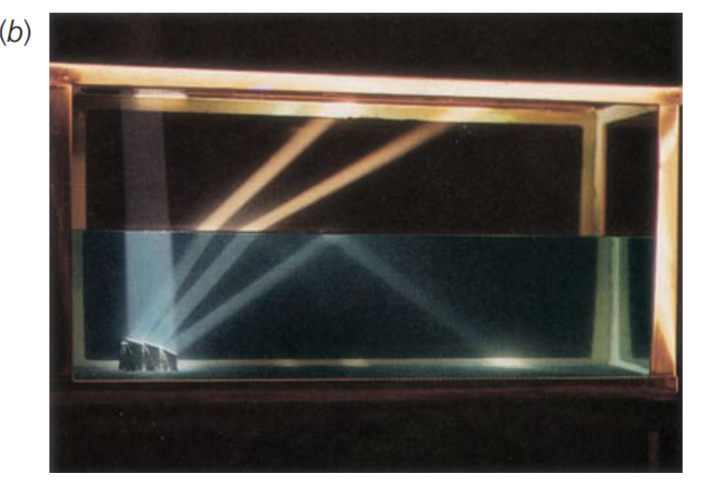
\includegraphics[width=8cm]{pic/kritis}
Pada peristiwa sudut kritis, sinar datang dari kerapatan tinggi $n_2$ ke $n_1$.
\begin{align*}
n_2.\sin(\theta_{\text{kritis}}) &=n_1.\sin(90)\\
n_2.\sin(\theta_{\text{kritis}}) &=n_1
\end{align*}


\item Indeks bias gelas adalah 1,5 dan indeks bias air 1,2. Sudut kritis bidang batas air-gelas adalah . . .
\pilgani{
        \item 30$^o$
        \item 45$^o$
        \item 53$^o$
        \item 60$^o$
        \item 75$^o$
        }
\vspace{3cm}
\item Suatu lapisan kimia dengan n = 1,5 ketebalan 6 cm mengapung di atas air (n = 1,33) dengan ketebalan 4 cm. Jarak semu antara dasar bejana dan permukaan lapisan kimia jika dipandang secara tegaklurus dari atas adalah  . . . 
\pilgani{
        \item 2 cm
        \item 5 cm
        \item 7 cm
        \item 10 cm
        \item 15 cm
        }
\vspace{3cm}


\textbf{INTERFERENSI CELAH GANDA}

Celah ganda menyebabkan adanya interferensi pada titik tertentu saat beda fasenya 1/2 gelombang. Satu sumber sejajar melewati dua celah sempit (\textit{slit}) dengan jarak $d$, ditangkap pada layar sejauh $L$ dari celah tersebut.

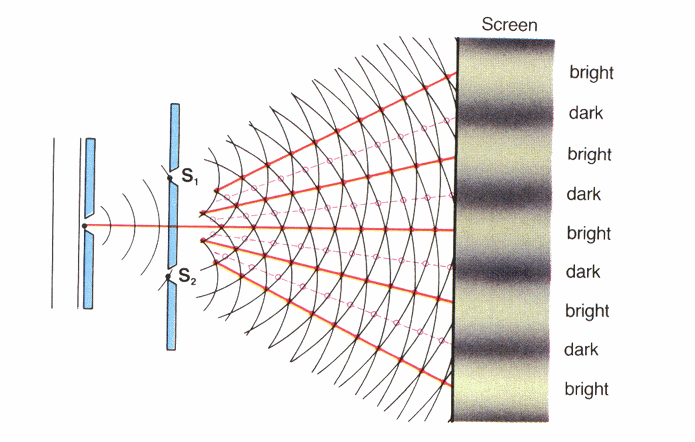
\includegraphics[width=8cm]{pic/interganda}

pola gelap terang akan selalu tetap seperti pada gambar, sehingga dapat ditulis dalam persamaan
\begin{align*}
\frac{dy}{L} &= n \lambda\\
d \sin (\theta) &= n \lambda
\end{align*}
$d$ : jarak antar celah\\
$y$ : jarak TERANG ke-$n$ dari TERANG PUSAT\\
$L$ : jarak celah ke layar\\ 
$n$ : orde terang ke - (misal 1,2,3, dst)\\


\item Cahaya dengan panjang gelombang 5000 $\r{A}$ datang pada celah kembar Young yang jaraknya 0,2 mm. Pola yang terjadi ditangkap pada layar yang jaraknya 1 m dari celah kembar. Jarak dari terang pusat ke terang yang paling pinggir pada layar = 2,5 cm. Banyaknya garis terang pada layar adalah . . . garis
\pilgani{
        \item 5
        \item 10
        \item 11
        \item 20
        \item 21
        }

\vspace{3cm} \item Dua panjang gelombang digunakan dalam percobaan Young. Jika salah satu panjang gelombangnya 480 nm, berapakah panjang gelombang lainnya supaya pita terang keempat cahaya yang pertama bertepatan dengan pita terang keenam dari cahaya lainnya?  \pilgani{
        \item 160 nm
        \item 240 nm
        \item 320 nm
       \item 400 nm
        \item 480 nm
} \vspace{3cm} 


\textbf{DIFRAKSI CELAH TUNGGAL}

Pada proses difraski cahaya mengitari halangan kecil pada arah rambatnya, juga dapat menyebar keluar dari celah sempit. Proses difraksi mirip dengan interferensi (lihat gambar). Namun pola terangnya tidak tetap. Oleh karena itu pada difraksi yang dihitung pada orde ke-$n$ adalah pola gelap ke $n$. 

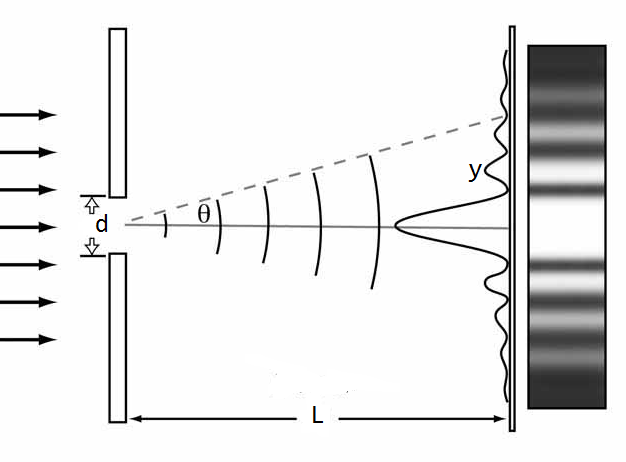
\includegraphics[width=6cm]{pic/singleslit}
\begin{align*}
\frac{dy}{L} &= n \lambda\\
d \sin (\theta) &= n \lambda
\end{align*}
$d$ : jarak antar celah\\
$y$ : jarak GELAP ke-$n$ dari TERANG PUSAT\\
$L$ : jarak celah ke layar\\ 
$n$ : orde gelap ke - (misal 1,2,3, dst)\\



\item Celah tunggal selebar 0,1 mm disinari berkas cahaya sejajar dengan $\lambda = 6000 \r{A}$. Pola difraksi yang terjadi ditangkap oleh layar pada jarak 40 cm dari celah. Jarak antara pita gelap ketiga dengan titik tengah gelap pusat pada layar adalah . . . .
\pilgani{
        \item 1,6 mm
        \item 3,2 mm
        \item 3,6 mm
        \item 7,2 mm
        \item 9,6 mm
        }

\vspace{3cm}

\textbf{DIFRAKSI KISI}\\
Kisi difraksi adalah suatu alat yang terbuat dari pelat logam atau kaca yang pada permukaannya digoreskan garis-garis sejajar dengan jumlah sangat besar.

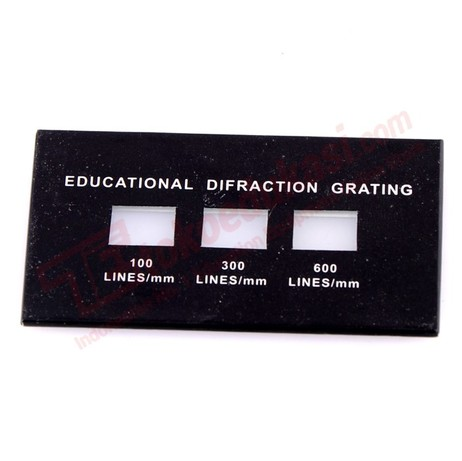
\includegraphics[width=6cm]{pic/kisi2}

Persamaan Kisi Difraksi mirip dengan persamaan interferensi celah ganda. Namun pada kisi difraksi besarnya $d$ tidak langsung diketahui, lihat pada gambar paling kiri. Banyaknya garis adalah 100 garis tiap mm. Maka jarak $d$ antar celah adalah
\begin{align*}
d &= \frac{1}{N}\\
d &=\frac{1 \text{ mm}}{100}\\
d &=\frac{ 10^{-3}}{100}=10^{-4}\text{ m}
\end{align*}
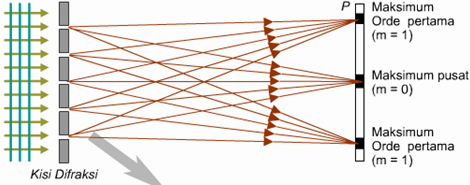
\includegraphics[width=8cm]{pic/kisi}\\
\begin{align*}
\frac{dy}{L} &= n \lambda\\
d \sin (\theta) &= n \lambda
\end{align*}
$d$ : jarak antar celah\\
$y$ : jarak TERANG ke-$n$ dari TERANG PUSAT\\
$L$ : jarak celah ke layar\\ 
$n$ : orde terang ke - (misal 1,2,3, dst)\\


\item Seberkas cahaya monokromatik dengan panjang gelombang 600 nm menyinari tegak lurus suatu kisi yang terdiri dari 500 garis /mm. Tentukan sudut deviasi orde kkedua!  \pilgani{ \item 30$^o$
        \item 37$^o$
        \item 45$^o$
        \item 53$^o$
        \item 60$^o$
        }

\vspace{2cm}






\textbf{POLARISASI CAHAYA}\\
\begin{align*}
 I_1 &= \frac{1}{2} I_o\\
I_2 &= \cos^2 (\theta) I_1 = \frac{1}{2}\cos^2(\theta) I_o
\end{align*}
$I_o$ : intensitas cahaya tak terpolarisasi\\
$I_1$ : intensitas cahaya setelah dipolarisasi\\
$I_2$ : intensitas keluar analisator 

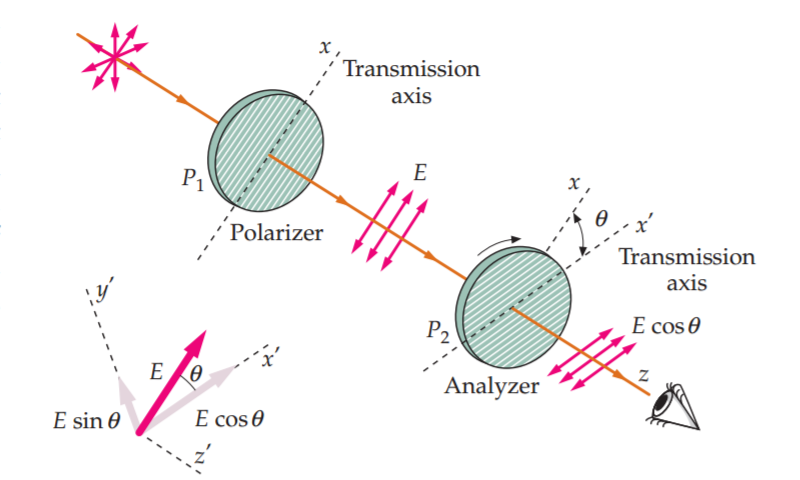
\includegraphics[width=8cm]{pic/polarisasi}
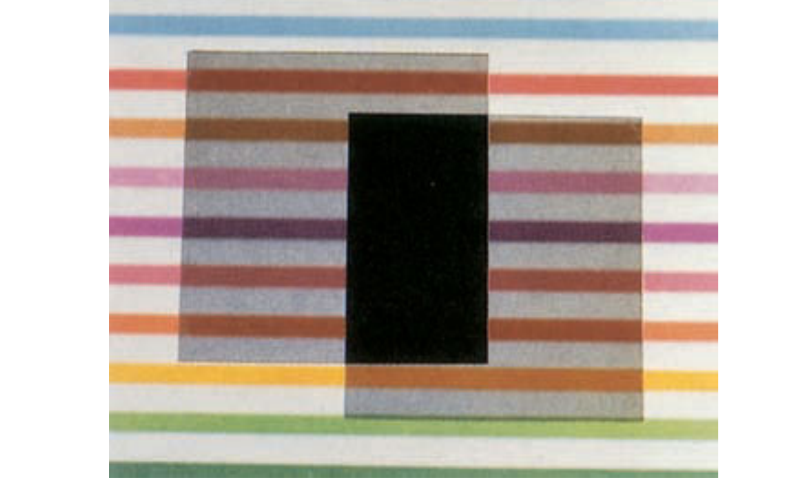
\includegraphics[width=8cm]{pic/polarisasi2}

\item Sinar tak terpolarisasi dengan intensitas I datang pada polariod dari 2 lembar polaroid ideal. Berapakah seharusnya sudut antara sumbu-sumbu polarisasi dari kedua polaroid, jika intensitas besar cahaya yang keluar adalah $\frac{I}{4}$?
\pilgani{
        \item 30 $^o$
        \item 37 $^o$
        \item 45$^o$
        \item 53$^o$
        \item 60$^o$
        }
\vspace{2cm}
\item Sinar sejajar (terpolarisasi) dengan intensitas 2$\times 10^{-4}$ W/m$^2$ ke arah vertikal merambat pada analisator pada sudut 45$^o$ terhadap sumbu-$x$. Maka intensitas pada saat keluar dari analisator adalah . . . 
\pilgani{
        \item 1$\times 10^{-4}$ W/m$^2$
        \item 0,75$\times 10^{-4}$ W/m$^2$
        \item 2$\sqrt{3}\times 10^{-4}$ W/m$^2$
        \item 2$\sqrt{2}\times 10^{-4}$ W/m$^2$
        \item $\sqrt{2}\times 10^{-4}$ W/m$^2$
        }
\vspace{2cm}
        
\textbf{PEMBIASAN PADA PERMUKAAN LENGKUNG}
\graphicspath{ {pic/} }
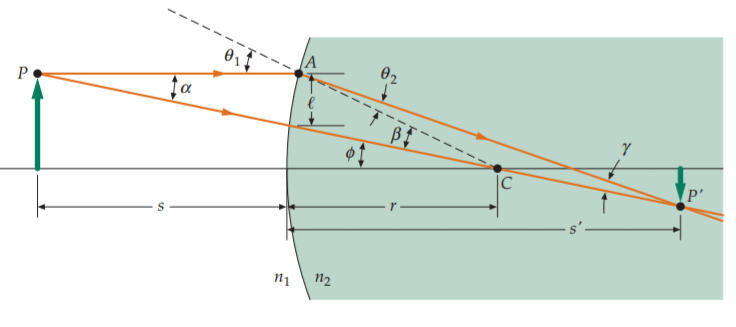
\includegraphics[width=8cm]{rumuslensasingle}
\begin{align*}
\frac{n_1}{s}+\frac{n_2}{s'}&=\frac{n_2-n_1}{r}
\end{align*}

\item Jari-jari salah satu ujung permukaan sebuah silinder kaca (n=1,5) setengah bola adalah 2 cm. Benda dengan tinggi 2 mm ditempatkan pada jarak 8 cm dari permukaan itu. Jarak bayangan bila silinder kaca itu cembung adalah . . .
\pilgani{
        \item 12 cm
        \item 20 cm
        \item 24 cm
        \item 36 cm
        \item 40 cm
        }

\textbf{LENSA TIPIS}\\
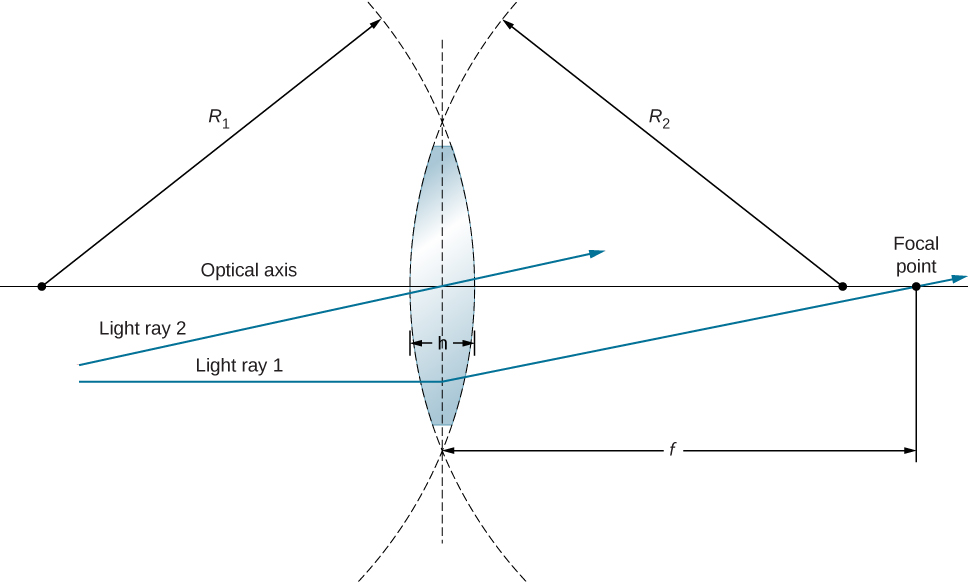
\includegraphics[width=8cm]{thin}
\begin{align*}
\frac{1}{f}&= \left ( \frac{n_2}{n_1} -1 \right) \left( \frac{1}{R_2}+\frac{1}{R_1} \right )
\end{align*}

\item Jarak fokus lensa gelas ( n = 1,5 ) di dalam alkohol ( n = 1,35) adalah 45 cm. Hitung jarak fokus dan kuat lensa tersebut di udara . . .
\pilgani{
        \item 10 cm dan 10 
        \item 20 cm dan 5
        \item 50 cm dan 2
        \item 40 cm dan 2,5
        \item 100 cm dan 1
        }


\end{enumerate}

\end{multicols*}\end{document}






